\documentclass[a4paper,12pt]{article}
\usepackage[spanish]{babel}
\usepackage[utf8]{inputenc}
\usepackage[T1]{fontenc}
\usepackage{graphicx}
\usepackage[pdftex,colorlinks=true, pdfstartview=FitH, linkcolor=blue,
citecolor=blue, urlcolor=blue, pdfpagemode=UseOutlines, pdfauthor={H. Asorey},
pdftitle={Física Moderna A - Asorey - 2017}]{hyperref}
\usepackage[adobe-utopia]{mathdesign}

\hoffset -1.23cm
\textwidth 16.5cm
\voffset -2.0cm
\textheight 26.0cm

%----------------------------------------------------------------
\begin{document}
\title{
{\normalsize{Universidad Nacional de Río Negro - Profesorados de Física}}\\
Física Moderna A \\ Segundo Parcial\\}
\author{Asorey}
\date{2017}
\maketitle

{\bf{Notas}}:
\begin{enumerate}
	\item Cuando corresponda, puede ({\textit{debe}}) utilizar resultados y
		expresiones de clase y de las guías. No es necesario volver a calcular
		todo ni copiarlas. Con sólo decir esta ecuación se calculó en tal clase
		o guía es suficiente.
	\item Las respuestas de cada ejercicio planteado deberán ser cargadas en un
		formulario en línea que será oportunamente informado. Allí deberá
		colocar los resultados numéricos y justificaciones (según corresponda).
		Luego, deberá escanear o fotografiar todos los desarrollos y subirlos
		en un documento pdf o zip al enviar el formulario.
	\item Se recibirán parciales hasta el Martes 27/Junio a las 23:59:59. El
		formulario se cierra en forma automática y por lo tanto, no se
		recibirán respuestas pasada la fecha límite. 
	\item El tiempo de resolución de este parcial se estima en 3 horas de
		trabajo continuo. 
	\item Ambos problemas tienen el mismo valor.
\end{enumerate}

{\bf{Ejercicios}}:
\begin{enumerate}
	\item {\bf{Pozo y barrera}}:\\
		Sea un electrón con masa $m$ y energía $E$ en un pozo de potencial
		finito de ancho $L=0.5$\,nm, donde las paredes del pozo tienen un ancho
		de $a=0.1$\,nm, tal como se muestra en la figura \ref{fig1}. La energía
		de la barrera de potencial $U_0$ puede ser modificada a voluntad, es
		decir, $U_0 = j E_\infty$, donde $j$ es un número natural y $E_\infty$
		corresponde a la energía del nivel fundamental de un pozo infinito del
		mismo ancho. Si inicialmente se fija $j=5$ y la energía del electrón es
		$E=3 E_\infty$, entonces:
		\begin{enumerate}
			\item calcule, en eV, el valor de $E_\infty$, de $U_0$ y de $E$;
			\item Dibuje en forma aproximada y sin hacer ningún cálculo, la
				función de onda en las regiones I, II, III, IV, y V. Sólo haga
				el dibujo y puede usar la figura \ref{fig1} como base. ¿Dónde
				espera un comportamiento de partícula libre? ¿Cuál es la región
				clásicamente prohibida? ¿Qué tipo de comportamiento espera para
				la función de onda en dicha zona?
			\item Utilizando la expresión del problema 44 (guía 04), calcule la
				probabilidad de que el electrón escape de la barrera por cada
				lado, y cual es la probabilidad total de encontrar al electrón
				fuera del pozo de potencial.
			\item Considerando sólo el factor exponencial de la probabilidad de
				transmisión, $e^{-2\beta L}$, calcule la probabilidad de
				transmisión para los casos $j=6$, $j=4$, $j=3$ y $j=2$ e
				interprete en cada caso los resultados obtenidos, en
				particular, que ocurre cuando $U_0 \to E$ y $U_0<E$.
		\end{enumerate}
		\begin{figure}\label{fig1}
			\begin{center}
			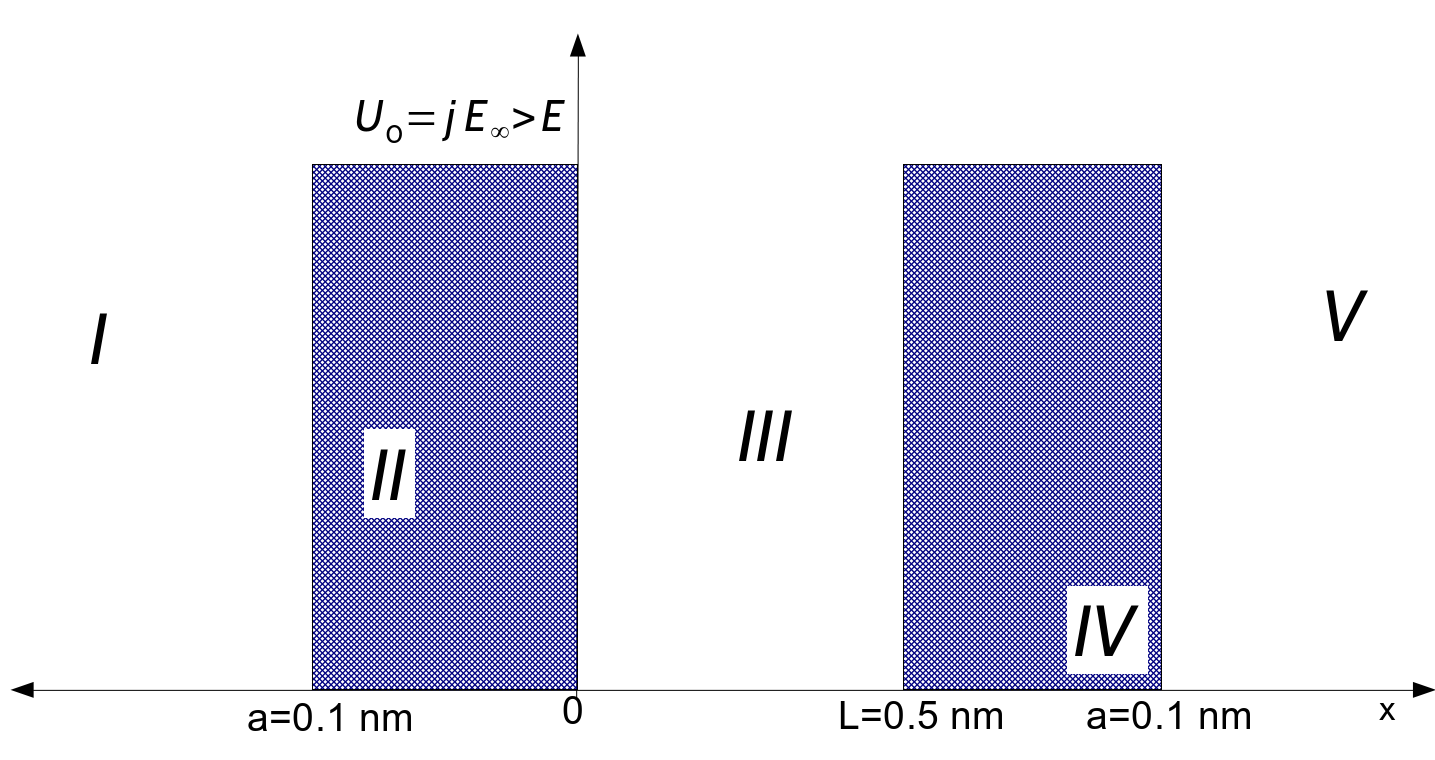
\includegraphics[width=0.7\textwidth]{../materiales/barrera.png}
			\end{center}
			\caption{{\bf{Barrera de potencial correspondiente al ejercicio 1}}.}
		\end{figure}

	\item {\bf{Alguna línea de Lyman}}:\\
		Sea un átomo de hidrógeno con el electrón en el
		nivel fundamental que absorbe un fotón con $\lambda=102.6$\,nm y momento
		angular $L_\gamma = + 1 \hbar$.
		\begin{enumerate}
			\item Calcule la energía del fotón absorbido y la energía del
				orbital inicial y final del electrón.
			\item Diga cuáles son los números cuánticos ($n_i$, $l_i$ y $m_i$)
				del electrón en el estado inicial, escriba la función de onda
				correspondiente a este estado, $\psi(r,\theta,\phi)$, y diga a
				que distancia del núcleo será más probable encontrar al
				electrón. Finalmente, mencione si es posible o no (no hace
				falta hacer el cálculo detallado), encontrar al electrón más
				allá del punto de retorno clásico. Justifique.
			\item A partir de la conservación del momento angular, diga cuál es
				el cambio total del $L$ del sistema y, usando las reglas de
				selección, diga cuales son los posibles números cuánticos del
				electrón en el estado final ($n_f$, $l_f$ y $m_f$) teniendo en
				cuenta las reglas de selección.
			\item Utilizando notación espectroscópica, escriba los posibles
				estados finales y las correspondientes funciones de onda
				$\psi_{n,l,m}$.
			\item A partir de las reglas de selección, enumere todos los
				posibles caminos que el electrón puede seguir para volver al
				nivel fundamental.
		\end{enumerate}
\end{enumerate}
\end{document}
